
The generalized extreme value distribution (GEV) includes all three
types of extreme value distributions: Type I (Gumbel), type II
(Fr\'{e}chet), and type III (Weibull). Empirically, the scores of some
sequence alignment algorithms appear to follow GEV distributions.  The
\eslmod{gev} module is used in estimating the statistical significance
of such scores.

Most local sequence alignment scores follow the Gumbel distribution.
Easel's \eslmod{gumbel} module applies specifically to the Gumbel. The
\eslmod{gev} module is used for Type II or III extreme value
distributions, or for determining which of the three types of
distribution that a dataset best fits.

\subsection{The gev API}

The \eslmod{gev} API consists of the following functions:

\vspace{0.5em}
\begin{center}
\begin{tabular}{ll}\hline
    \multicolumn{2}{c}{\textbf{evaluating densities and distributions:}}\\
\ccode{esl\_gev\_pdf()}     & Returns the probability density, $P(S=x)$.\\
\ccode{esl\_gev\_logpdf()}  & Returns the log of the pdf, $\log P(S=x)$.\\
\ccode{esl\_gev\_cdf()}     & Returns the cumulative probability distribution, $P(S \leq x)$.\\
\ccode{esl\_gev\_logcdf()}  & Returns the log of the cdf, $\log P(S \leq x)$.\\
\ccode{esl\_gev\_surv()}    & Returns right tail mass, 1-cdf, $P(S > x)$\\
\ccode{esl\_gev\_logsurv()} & Returns log of 1-cdf, $\log P(S > x)$.\\
    \multicolumn{2}{c}{\textbf{sampling:}}\\
\ccode{esl\_gev\_Sample()}  & Returns a GEV-distributed random sample.\\
    \multicolumn{2}{c}{\textbf{maximum likelihood parameter fitting:}}\\
\ccode{esl\_gev\_FitComplete()} & Estimates GEV parameters from complete data.\\
\end{tabular}
\end{center}
\vspace{0.5em}

The Gumbel distribution depends on three parameters, $\mu$, $\lambda$,
and $\alpha$. When these parameters are known, the statistical
significance (P-value) of a single score $x$ is $P(S>x)$, obtained by
a call to \ccode{esl\_gev\_surv()}.  The E-value for obtaining that
score or better in searching a database of $N$ sequences is just
$NP(S>x)$.

When the parameters are unknown, they can be estimated from scores
obtained from comparisons of simulated random data. The
\ccode{esl\_gev\_FitComplete()} function performs maximum likelihood
parameter fitting \citep{Coles01}.

\subsubsection{Augmentations: random, minimizer}

The \ccode{esl\_gev\_Sample()} function requires augmenting with the
\eslmod{random} module.

The \ccode{esl\_gev\_FitComplete()} function requires augmenting with
the \eslmod{minimizer} module.

\subsection{Example of using the gev API}

Below is a code example that samples 10,000 data points from a
Fr\'{e}chet distribution with $\mu=-20$, $\lambda=0.4$, $\alpha=0.1$;
reports the min and max samples, and the probability mass to the left
of the min and to the right of the max (both of which should be about
$\frac{1}{10000}$, since we took 10,000 samples); and then fits those
simulated data to a Gumbel and reports the fitted $\mu$ and $\lambda$:

\input{cexcerpts/gev_example}

\subsection{GEV densities}

The probability density function (pdf) and the cumulative distribution
function (cdf) of the generalized extreme value distribution are
\citep{Coles01}:

\begin{eqnarray}
P(X=x) & = & \lambda \left[ 1 + \alpha \lambda (x - \mu) \right]^{-\frac{\alpha+1}{\alpha}}
       \exp \left\{ - \left[ 1 + \alpha \lambda (x - \mu)
       \right]^{-\frac{1}{\alpha}} \right\} 
\\%
\label{eqn:gev_density}
P(X \geq x) & = & \exp \left\{ - \left[ 1 +
     \alpha\lambda(x-\mu) \right]^{-\frac{1}{\alpha}} \right\} 
\\%
\label{eqn:gev_distribution}
\end{eqnarray}

The parameters $\mu$, $\lambda$, and $\alpha$ are location, scale, and
shape parameters, respectively, with $-\infty < \mu < \infty$, $0 <
\lambda < \infty$, and $-\infty < \alpha < \infty$.

The Type II (Fr\'{e}chet) distribution corresponds to $\alpha > 0$,
and the Type III (Weibull) distribution corresponds to $\alpha < 0$.
The Type I (Gumbel) distribution arises in the limit $\alpha
\rightarrow 0$. At values $\alpha \simeq 0$, Easel's GEV functions
revert to the Gumbel limit case, as opposed to dividing by zero and
failing.

Technically the GEV is only defined for values of $x$ such that $1 +
\alpha \lambda (x - \mu) > 0$. However, Easel's functions return
sensible values outside this domain, such as 0 for nonexistent
densities.

Generalized extreme value densities for $\mu = 0$ and $\lambda = 1$
are shown below (left) for three settings of $\alpha$; $\alpha = 0$
(Gumbel), $\alpha = 0.1$ (Fr\'{e}chet), and $\alpha = -0.1$
(Weibull). The figure on the right shows the log densities, which more
clearly show how, relative to the exponential right tail of the
Gumbel, the Fr\'{e}chet's tail is longer, and the Weibull's tail is
shorter.

\centerline{
\begin{minipage}{3in}
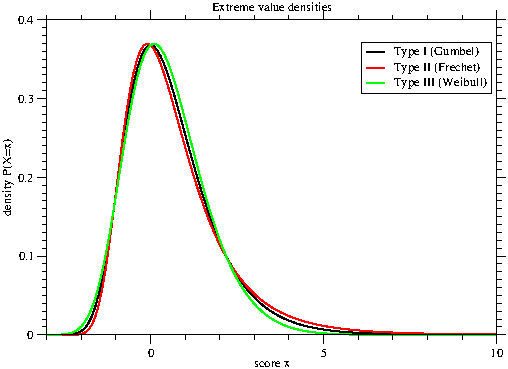
\includegraphics[width=2.8in]{figures/gev_density}
\end{minipage}
\begin{minipage}{3in}
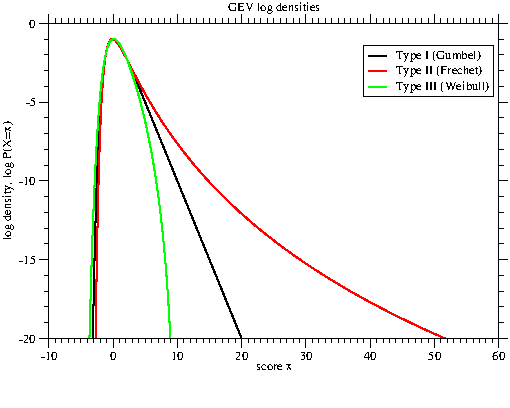
\includegraphics[width=2.8in]{figures/gev_logdensity}
\end{minipage}
}

For more details, see the excellent description in \citep{Coles01}.
Easel's $\{ \mu, \lambda, \alpha \}$ notation differs from the $\{
\mu, \sigma, \xi \}$ parameterization used by Coles. Use $\lambda =
\frac{1}{\sigma}$ and $\alpha = \xi$ to translate.

\subsection{Fitting GEV distributions to observed data}

Easel fits GEVs by maximum likelihood estimation by numerically
optimizing the log likelihood function, using first derivative
information and conjugate gradient descent.  See the \eslmod{gumbel}
chapter for a more general introduction to maximum likelihood fitting.

\subsubsection{Maximum likelihood estimation, complete data}

The function \ccode{esl\_gev\_FitComplete()} uses gradient information
to find parameters that optimize the likelihood function, using the
conjugate gradient descent code in the \eslmod{minimizer} module.

Given $n$ samples $x_1..x_n$, we want to estimate maximum likelihood
parameter estimates $\{ \hat{\mu}, \hat{\lambda}, \hat{\alpha} \}$
that maximize the log likelihood:

\begin{equation}
\log L(\lambda, \mu, \alpha) = n \log \lambda 
       - \frac{\alpha+1}{\alpha} 
           \sum_{i=1}^{n} \log\left[1+ \alpha\lambda(x_i - \mu) \right]
       - \sum_{i=1}^{n} \left[ 1 + \alpha\lambda (x_i - \mu) \right]^{\frac{1}{\alpha}}
\label{eqn:gev_logL}
\end{equation}

The $\left[ 1 + \alpha\lambda (x_i - \mu) \right]^{\frac{1}{\alpha}}$
term can be rewritten in a more conveniently differentiable form as
$\exp \left\{ \frac{1}{\alpha} \log \left[ 1 + \alpha\lambda (x_i - \mu)
\right] \right\}$.

Since the $\lambda$ parameter is constrained to $\lambda > 0$ but the
numerical optimizer expects unconstrained parameters, we use a change
of variables $\lambda = e^w$ and optimize an unconstrained value $w$.

The gradient of the log likelihood with respect to $\mu$, $w$, and
$\alpha$ is:

%% xref: STL9/118-120
\begin{eqnarray}
\frac{\partial \log L}{\partial \mu} & = &
  \sum_{i=1}^n \frac{\lambda (\alpha+1)}{1+\alpha\lambda(x_i-\mu)} 
 -\sum_{i=1}^n \lambda \exp 
    \left\{ -\frac{\alpha+1}{\alpha} \log
          \left[1+\alpha\lambda(x_i-\mu)\right] \right\}
\\%
\label{eqn:gev_mupartial}
\frac{\partial \log L}{\partial w} & = &
  n - \sum_{i=1}^{n} \frac{\lambda (\alpha+1) (x_i - \mu)} 
                          {1 + \alpha \lambda (x_i - \mu)}
  + \sum_{i=1}^n \lambda (x_i - \mu) 
         \exp \left\{ -\frac{\alpha+1}{\alpha} \log
          \left[1+\alpha\lambda(x_i-\mu)\right] \right\}
\\%
\label{eqn:gev_wpartial}
\frac{\partial \log L}{\partial \alpha} & = &
   \sum_{i=1}^n \left\{
      \begin{array}{l}
      - \frac{\alpha+1}{\alpha} \frac{\lambda(x_i-\mu)}
                                  {1 +\alpha\lambda(x_i-\mu)}\\
      + \frac{1}{\alpha^2} \log \left[ 1 + \alpha\lambda(x_i - \mu) \right]\\
      + \frac{1}{\alpha} \frac{\lambda(x_i-\mu)}
                          {1 +\alpha\lambda(x_i-\mu)}
      e^{-\frac{1}{\alpha} \log\left[ 1 + \alpha\lambda(x_i - \mu) \right]}\\
     -  \frac{1}{\alpha^2} \log \left[ 1 + \alpha\lambda(x_i - \mu) \right]
      e^{-\frac{1}{\alpha} \log\left[ 1 + \alpha\lambda(x_i - \mu)
	 \right]} 
     \end{array}
     \right.
\\%
\label{eqn:gev_alphapartial}
\end{eqnarray}

When $|\alpha\lambda(x_i - \mu)|$ approaches $0$, the GEV approximates
a Gumbel distribution and these equations can be simplified using the
approximation $\log(1+a) \simeq a$.







